% Options for packages loaded elsewhere
\PassOptionsToPackage{unicode}{hyperref}
\PassOptionsToPackage{hyphens}{url}
%
\documentclass[
]{book}
\usepackage{lmodern}
\usepackage{amssymb,amsmath}
\usepackage{ifxetex,ifluatex}
\ifnum 0\ifxetex 1\fi\ifluatex 1\fi=0 % if pdftex
  \usepackage[T1]{fontenc}
  \usepackage[utf8]{inputenc}
  \usepackage{textcomp} % provide euro and other symbols
\else % if luatex or xetex
  \usepackage{unicode-math}
  \defaultfontfeatures{Scale=MatchLowercase}
  \defaultfontfeatures[\rmfamily]{Ligatures=TeX,Scale=1}
\fi
% Use upquote if available, for straight quotes in verbatim environments
\IfFileExists{upquote.sty}{\usepackage{upquote}}{}
\IfFileExists{microtype.sty}{% use microtype if available
  \usepackage[]{microtype}
  \UseMicrotypeSet[protrusion]{basicmath} % disable protrusion for tt fonts
}{}
\makeatletter
\@ifundefined{KOMAClassName}{% if non-KOMA class
  \IfFileExists{parskip.sty}{%
    \usepackage{parskip}
  }{% else
    \setlength{\parindent}{0pt}
    \setlength{\parskip}{6pt plus 2pt minus 1pt}}
}{% if KOMA class
  \KOMAoptions{parskip=half}}
\makeatother
\usepackage{xcolor}
\IfFileExists{xurl.sty}{\usepackage{xurl}}{} % add URL line breaks if available
\IfFileExists{bookmark.sty}{\usepackage{bookmark}}{\usepackage{hyperref}}
\hypersetup{
  pdftitle={Basic Stats},
  pdfauthor={Bill Last Updated:},
  hidelinks,
  pdfcreator={LaTeX via pandoc}}
\urlstyle{same} % disable monospaced font for URLs
\usepackage{color}
\usepackage{fancyvrb}
\newcommand{\VerbBar}{|}
\newcommand{\VERB}{\Verb[commandchars=\\\{\}]}
\DefineVerbatimEnvironment{Highlighting}{Verbatim}{commandchars=\\\{\}}
% Add ',fontsize=\small' for more characters per line
\usepackage{framed}
\definecolor{shadecolor}{RGB}{248,248,248}
\newenvironment{Shaded}{\begin{snugshade}}{\end{snugshade}}
\newcommand{\AlertTok}[1]{\textcolor[rgb]{0.94,0.16,0.16}{#1}}
\newcommand{\AnnotationTok}[1]{\textcolor[rgb]{0.56,0.35,0.01}{\textbf{\textit{#1}}}}
\newcommand{\AttributeTok}[1]{\textcolor[rgb]{0.77,0.63,0.00}{#1}}
\newcommand{\BaseNTok}[1]{\textcolor[rgb]{0.00,0.00,0.81}{#1}}
\newcommand{\BuiltInTok}[1]{#1}
\newcommand{\CharTok}[1]{\textcolor[rgb]{0.31,0.60,0.02}{#1}}
\newcommand{\CommentTok}[1]{\textcolor[rgb]{0.56,0.35,0.01}{\textit{#1}}}
\newcommand{\CommentVarTok}[1]{\textcolor[rgb]{0.56,0.35,0.01}{\textbf{\textit{#1}}}}
\newcommand{\ConstantTok}[1]{\textcolor[rgb]{0.00,0.00,0.00}{#1}}
\newcommand{\ControlFlowTok}[1]{\textcolor[rgb]{0.13,0.29,0.53}{\textbf{#1}}}
\newcommand{\DataTypeTok}[1]{\textcolor[rgb]{0.13,0.29,0.53}{#1}}
\newcommand{\DecValTok}[1]{\textcolor[rgb]{0.00,0.00,0.81}{#1}}
\newcommand{\DocumentationTok}[1]{\textcolor[rgb]{0.56,0.35,0.01}{\textbf{\textit{#1}}}}
\newcommand{\ErrorTok}[1]{\textcolor[rgb]{0.64,0.00,0.00}{\textbf{#1}}}
\newcommand{\ExtensionTok}[1]{#1}
\newcommand{\FloatTok}[1]{\textcolor[rgb]{0.00,0.00,0.81}{#1}}
\newcommand{\FunctionTok}[1]{\textcolor[rgb]{0.00,0.00,0.00}{#1}}
\newcommand{\ImportTok}[1]{#1}
\newcommand{\InformationTok}[1]{\textcolor[rgb]{0.56,0.35,0.01}{\textbf{\textit{#1}}}}
\newcommand{\KeywordTok}[1]{\textcolor[rgb]{0.13,0.29,0.53}{\textbf{#1}}}
\newcommand{\NormalTok}[1]{#1}
\newcommand{\OperatorTok}[1]{\textcolor[rgb]{0.81,0.36,0.00}{\textbf{#1}}}
\newcommand{\OtherTok}[1]{\textcolor[rgb]{0.56,0.35,0.01}{#1}}
\newcommand{\PreprocessorTok}[1]{\textcolor[rgb]{0.56,0.35,0.01}{\textit{#1}}}
\newcommand{\RegionMarkerTok}[1]{#1}
\newcommand{\SpecialCharTok}[1]{\textcolor[rgb]{0.00,0.00,0.00}{#1}}
\newcommand{\SpecialStringTok}[1]{\textcolor[rgb]{0.31,0.60,0.02}{#1}}
\newcommand{\StringTok}[1]{\textcolor[rgb]{0.31,0.60,0.02}{#1}}
\newcommand{\VariableTok}[1]{\textcolor[rgb]{0.00,0.00,0.00}{#1}}
\newcommand{\VerbatimStringTok}[1]{\textcolor[rgb]{0.31,0.60,0.02}{#1}}
\newcommand{\WarningTok}[1]{\textcolor[rgb]{0.56,0.35,0.01}{\textbf{\textit{#1}}}}
\usepackage{longtable,booktabs}
% Correct order of tables after \paragraph or \subparagraph
\usepackage{etoolbox}
\makeatletter
\patchcmd\longtable{\par}{\if@noskipsec\mbox{}\fi\par}{}{}
\makeatother
% Allow footnotes in longtable head/foot
\IfFileExists{footnotehyper.sty}{\usepackage{footnotehyper}}{\usepackage{footnote}}
\makesavenoteenv{longtable}
\usepackage{graphicx,grffile}
\makeatletter
\def\maxwidth{\ifdim\Gin@nat@width>\linewidth\linewidth\else\Gin@nat@width\fi}
\def\maxheight{\ifdim\Gin@nat@height>\textheight\textheight\else\Gin@nat@height\fi}
\makeatother
% Scale images if necessary, so that they will not overflow the page
% margins by default, and it is still possible to overwrite the defaults
% using explicit options in \includegraphics[width, height, ...]{}
\setkeys{Gin}{width=\maxwidth,height=\maxheight,keepaspectratio}
% Set default figure placement to htbp
\makeatletter
\def\fps@figure{htbp}
\makeatother
\setlength{\emergencystretch}{3em} % prevent overfull lines
\providecommand{\tightlist}{%
  \setlength{\itemsep}{0pt}\setlength{\parskip}{0pt}}
\setcounter{secnumdepth}{5}
\usepackage{booktabs}
\usepackage{amsthm}
\makeatletter
\def\thm@space@setup{%
  \thm@preskip=8pt plus 2pt minus 4pt
  \thm@postskip=\thm@preskip
}
\makeatother
\usepackage[]{natbib}
\bibliographystyle{apalike}

\title{Basic Stats}
\author{Bill Last Updated:}
\date{15 February, 2020}

\begin{document}
\frontmatter
\maketitle

{
\setcounter{tocdepth}{1}
\tableofcontents
}
\mainmatter
\hypertarget{my-section}{%
\chapter*{Preface: Motivation}\label{my-section}}
\addcontentsline{toc}{chapter}{Preface: Motivation}

All the notes I have done here are about basic stats. While I have tried my best, probably there are still some typos and errors. Please feel free to let me know in case you find one. Thank you!

\hypertarget{logit-and-probit}{%
\chapter{Logit and Probit}\label{logit-and-probit}}

\hypertarget{logit}{%
\section{Logit}\label{logit}}

\[f(x)=log(\frac{p(y=1)}{1-p(y=1)})\]
The basic idea of logistic regression:
\[p(y=1)=\frac{1}{1+e^{-(\beta_0+\beta_1x_1+...+\beta_nx_n)}}=\frac{e^{\beta_0+\beta_1x_1+...+\beta_nx_n}}{1+e^{\beta_0+\beta_1x_1+...+\beta_nx_n}}\]
Thus, \(e^{\beta_0+\beta_1x_1+...+\beta_nx_n}\) can be from \(-\infty\) to \(+\infty\), and \(p(y=1)\) will be always within the range of \((0,1)\).

\begin{Shaded}
\begin{Highlighting}[]
\NormalTok{f<-}\ControlFlowTok{function}\NormalTok{(x)\{}\KeywordTok{exp}\NormalTok{(x)}\OperatorTok{/}\NormalTok{(}\DecValTok{1}\OperatorTok{+}\KeywordTok{exp}\NormalTok{(x))\}}
\NormalTok{data<-}\KeywordTok{seq}\NormalTok{(}\OperatorTok{-}\DecValTok{10}\NormalTok{,}\DecValTok{10}\NormalTok{,}\DecValTok{1}\NormalTok{)}
\KeywordTok{plot}\NormalTok{(data,}\KeywordTok{f}\NormalTok{(data),}\DataTypeTok{type =} \StringTok{"b"}\NormalTok{)}
\end{Highlighting}
\end{Shaded}

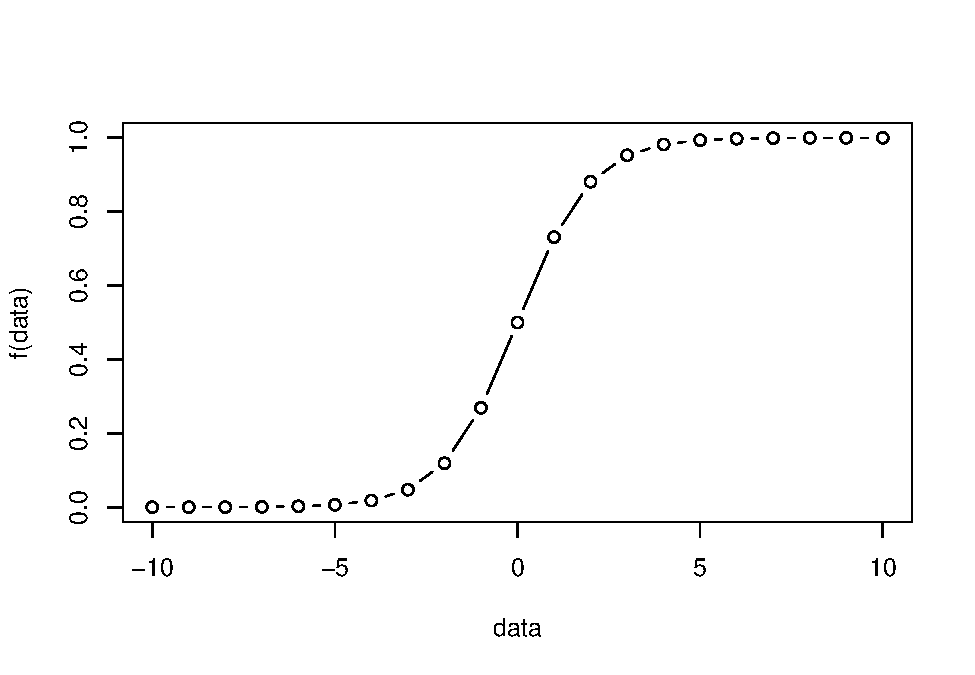
\includegraphics{bookdown-demo_files/figure-latex/unnamed-chunk-1-1.pdf}

We can also write the function into another format as follows:
\[log \frac{p(y=1)}{1-p(y=1)}= \beta_0+\beta_1x_1+...+\beta_nx_n\]
Thus, we know that the regression coeficients of \(\beta_i\) actually change the ``log-odds'' of the event. Of course, note that the magnitude of \(\beta_i\) is dependent upon the units of \(x_i\).

The following is an example testing whether that home teams are more likely to win in NFL games. The results show that the odd of winning is the same for both home and away teams.

\begin{Shaded}
\begin{Highlighting}[]
\NormalTok{mydata =}\StringTok{ }\KeywordTok{read.csv}\NormalTok{(}\KeywordTok{url}\NormalTok{(}\StringTok{'https://raw.githubusercontent.com/nfl-football-ops/Big-Data-Bowl/master/Data/games.csv'}\NormalTok{))}
\NormalTok{mydata}\OperatorTok{$}\NormalTok{result_new<-}\KeywordTok{ifelse}\NormalTok{(mydata}\OperatorTok{$}\NormalTok{HomeScore}\OperatorTok{>}\NormalTok{mydata}\OperatorTok{$}\NormalTok{VisitorScore,}\DecValTok{1}\NormalTok{,}\DecValTok{0}\NormalTok{)}
\KeywordTok{summary}\NormalTok{(mydata}\OperatorTok{$}\NormalTok{result_new)}
\end{Highlighting}
\end{Shaded}

\begin{verbatim}
##    Min. 1st Qu.  Median    Mean 3rd Qu.    Max. 
##  0.0000  0.0000  0.0000  0.4945  1.0000  1.0000
\end{verbatim}

\begin{Shaded}
\begin{Highlighting}[]
\NormalTok{mylogit1 =}\StringTok{ }\KeywordTok{glm}\NormalTok{(result_new}\OperatorTok{~}\DecValTok{1}\NormalTok{, }\DataTypeTok{family=}\NormalTok{binomial, }\DataTypeTok{data=}\NormalTok{mydata)}
\KeywordTok{summary}\NormalTok{(mylogit1)}
\end{Highlighting}
\end{Shaded}

\begin{verbatim}
## 
## Call:
## glm(formula = result_new ~ 1, family = binomial, data = mydata)
## 
## Deviance Residuals: 
##    Min      1Q  Median      3Q     Max  
## -1.168  -1.168  -1.168   1.187   1.187  
## 
## Coefficients:
##             Estimate Std. Error z value Pr(>|z|)
## (Intercept) -0.02198    0.20967  -0.105    0.917
## 
## (Dispersion parameter for binomial family taken to be 1)
## 
##     Null deviance: 126.14  on 90  degrees of freedom
## Residual deviance: 126.14  on 90  degrees of freedom
## AIC: 128.14
## 
## Number of Fisher Scoring iterations: 3
\end{verbatim}

\hypertarget{probit}{%
\section{Probit}\label{probit}}

As noted above, logit \(f(x)=log(\frac{p(y=1)}{1-p(y=1)})\) provides the resulting range of \((0,1)\). Another way to provide the same rage is through the cdf of normal distribution.The following R code is used to illusrate this process.

\begin{Shaded}
\begin{Highlighting}[]
\NormalTok{data2<-}\KeywordTok{seq}\NormalTok{(}\OperatorTok{-}\DecValTok{5}\NormalTok{,}\DecValTok{5}\NormalTok{,}\DecValTok{1}\NormalTok{)}
\KeywordTok{plot}\NormalTok{(data2,}\KeywordTok{pnorm}\NormalTok{(data2),}\DataTypeTok{type =} \StringTok{"b"}\NormalTok{)}
\end{Highlighting}
\end{Shaded}

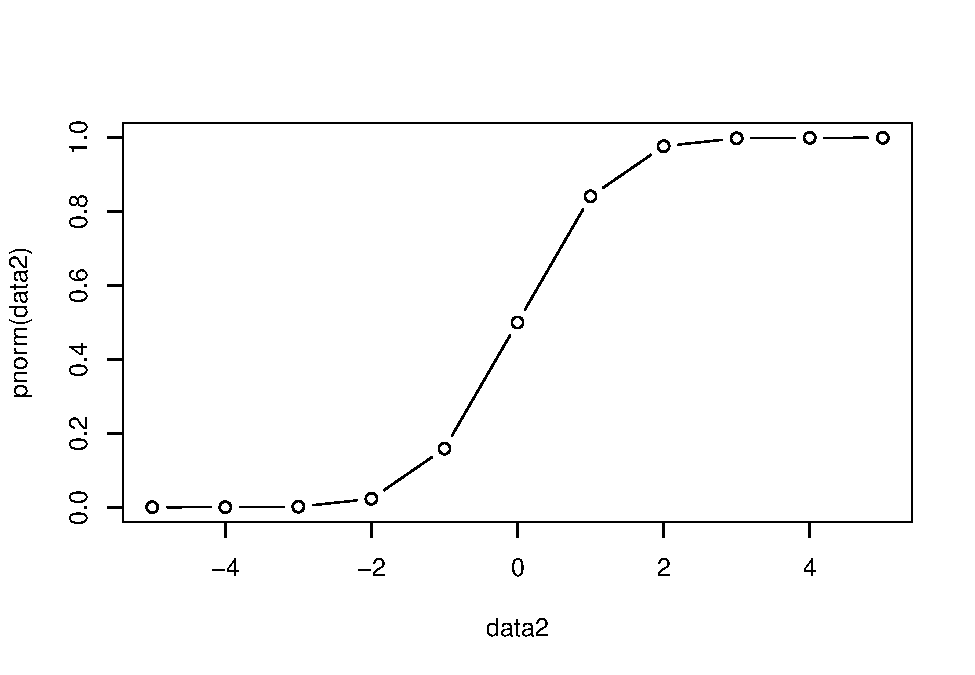
\includegraphics{bookdown-demo_files/figure-latex/unnamed-chunk-3-1.pdf}
Thus, the cdf of normal distribution can be used to indicate the probability of \(p(y=1)\).

\[\Phi(\beta_0+\beta_1x_1+...+\beta_nx_n )= p(y=1)\]

Similar to logit model, we can also write the inverse function of the cdf to get the function that can be from \(-\infty\) to \(+\infty\).

\[\beta_0+\beta_1x_1+...+\beta_nx_n =\Phi^{-1}(p(y=1))\]

Thus, for example, if \(X\beta\) = -2, based on \(\Phi(\beta_0+\beta_1x_1+...+\beta_nx_n )= p(y=1)\) we can get that the \(p(y=1)=0.023\).

In contrast, if \(X\beta\) = 3, the \(p(y=1)=0.999\).

\begin{Shaded}
\begin{Highlighting}[]
\KeywordTok{pnorm}\NormalTok{(}\OperatorTok{-}\DecValTok{2}\NormalTok{)}
\end{Highlighting}
\end{Shaded}

\begin{verbatim}
## [1] 0.02275013
\end{verbatim}

\begin{Shaded}
\begin{Highlighting}[]
\KeywordTok{pnorm}\NormalTok{(}\DecValTok{3}\NormalTok{)}
\end{Highlighting}
\end{Shaded}

\begin{verbatim}
## [1] 0.9986501
\end{verbatim}

Let's assume that there is a latent variable called \(Y^*\) such that

\[Y^*=X\beta+\epsilon, \epsilon \sim N(0,\sigma^2)\]
You could think of \(Y^*\) as a kind of ``proxy'' between \(X\beta+\epsilon\) and the observed \(Y (1 or 0)\). Thus, we can get the following. Note that, it does not have to be zero, and can be any constant.

\[
Y^*=\begin{cases} 0 \;\;\: if \;  y_i^* \leq 0 \\ 1 \;\;\: if \;  y_i^* > 0 \end{cases}
\]

Thus,

\[y_i^* > 0 \Rightarrow \beta^{'}X_i + \epsilon_i >0 \Rightarrow \epsilon_i > -\beta^{'}X_i\]

Thus, we can write it as follows. Note that \(\frac{ \epsilon_i}{\sigma} \sim N(0,1)\)

\[p(y=1|x_i)= p(y_i^* >0|x_i)=p(\epsilon_i > -\beta^{'}X_i)= p(\frac{ \epsilon_i}{\sigma}>\frac{-\beta^{'}X_i}{\sigma})=\Phi(\frac{\beta^{'}X_i}{\sigma}) \]
We thus can get:

\[p(y=0|x_i)=1-\Phi(\frac{\beta^{'}X_i}{\sigma})\]

For \(p(y=1|x_i)=\Phi(\frac{\beta^{'}X_i}{\sigma})\), we can not really estimate both \(\beta\) and \(\sigma\) as they are in a ratio. We can assume \(\sigma =1\), then \(\epsilon \sim N(0,1)\).
We know \(y_i\) and \(x_i\) since we observe them. Thus, we can write it as follows.

\[p(y=1|x_i)=\Phi(\beta^{'}X_i)\]

\hypertarget{intro}{%
\chapter{MLE}\label{intro}}

\hypertarget{basic-idea-of-mle}{%
\section{Basic idea of MLE}\label{basic-idea-of-mle}}

Suppose that we flip a coin, \(y_i=0\) for tails and \(y_i=1\) for heads. If we get \(p\) heads from \(n\) trials, we can get the proportion of heads is \(p/n\), which is the sample mean. If we do not do any further calculation, this is our best guess.

Suppose that the true proablity is \(\rho\), then we can get:

\[
\mathbf{L}(y_i)=\begin{cases} \rho \;\;\:   y_i = 1 \\ 1-\rho \;\;\:  y_i = 0 \end{cases}
\]
Thus, we can also write it as follows.
\[\mathbf{L}(y_i) = \rho^{y_i}(1-\rho)^{1-y_i}\]

Thus, we can get:

\[\prod \mathbf{L}(y_i|\rho)=\rho^{\sum y_i}(1-\rho)^{\sum(1-y_i)}\]
Further, we can get a log-transformed format.

\[log (\prod \mathbf{L}(y_i|\rho))=\sum y_i log \rho + \sum(1-y_i) log(1-\rho)\]

To maximize the log-function above, we can calculate the derivative with respect to \(\rho\).
\[\frac{\partial log (\prod \mathbf{L}(y_i|\rho)) }{\partial \rho}=\sum y_i \frac{1}{\rho}-\sum(1-y_i) \frac{1}{1-\rho}\]
Set the derivative to zero and solve for \(\rho\), we can get

\[\sum y_i \frac{1}{\rho}-\sum(1-y_i) \frac{1}{1-\rho}=0\]
\[\Rightarrow (1-\rho)\sum y_i - \rho \sum(1-y_i) =0\]
\[\Rightarrow \sum y_i-\rho\sum y_i - n\rho +\rho\sum y_i =0\]
\[\Rightarrow \sum y_i - n\rho  =0\]
\[\Rightarrow \rho  = \frac{\sum y_i}{n}=\frac{p}{n}\]
Thus, we can see that the \(\rho\) maximizing the likelihood function is equal to the sample mean.

\hypertarget{coin-flip-example-probit-and-logit}{%
\section{Coin flip example, probit, and logit}\label{coin-flip-example-probit-and-logit}}

In the example above, we are not really trying to estimate a lot of regression coefficients. What we are doing actually is to calculate the sample mean, or intercept in the regresion sense. What does it mean? Let's use some data to explain it.

Suppose that we flip a coin 20 times and observe 8 heads. We can use the R's glm function to esimate the \(\rho\). If the result is consistent with what we did above, we should observe that the \(cdf\) of the esimate of \(\beta_0\) (i.e., intercept) should be equal to \(8/20=0.4\).

\begin{Shaded}
\begin{Highlighting}[]
\NormalTok{coins<-}\KeywordTok{c}\NormalTok{(}\KeywordTok{rep}\NormalTok{(}\DecValTok{1}\NormalTok{,}\DataTypeTok{times=}\DecValTok{8}\NormalTok{),}\KeywordTok{rep}\NormalTok{(}\DecValTok{0}\NormalTok{,}\DataTypeTok{times=}\DecValTok{12}\NormalTok{))}
\KeywordTok{table}\NormalTok{(coins)}
\end{Highlighting}
\end{Shaded}

\begin{verbatim}
## coins
##  0  1 
## 12  8
\end{verbatim}

\begin{Shaded}
\begin{Highlighting}[]
\NormalTok{coins<-}\KeywordTok{as.data.frame}\NormalTok{(coins)}
\end{Highlighting}
\end{Shaded}

\hypertarget{probit-1}{%
\subsection{Probit}\label{probit-1}}

\begin{Shaded}
\begin{Highlighting}[]
\NormalTok{probitresults <-}\StringTok{ }\KeywordTok{glm}\NormalTok{(coins }\OperatorTok{~}\StringTok{ }\DecValTok{1}\NormalTok{, }\DataTypeTok{family =} \KeywordTok{binomial}\NormalTok{(}\DataTypeTok{link =} \StringTok{"probit"}\NormalTok{), }\DataTypeTok{data =}\NormalTok{ coins)}
\NormalTok{probitresults}
\end{Highlighting}
\end{Shaded}

\begin{verbatim}
## 
## Call:  glm(formula = coins ~ 1, family = binomial(link = "probit"), 
##     data = coins)
## 
## Coefficients:
## (Intercept)  
##     -0.2533  
## 
## Degrees of Freedom: 19 Total (i.e. Null);  19 Residual
## Null Deviance:       26.92 
## Residual Deviance: 26.92     AIC: 28.92
\end{verbatim}

\begin{Shaded}
\begin{Highlighting}[]
\KeywordTok{pnorm}\NormalTok{(probitresults}\OperatorTok{$}\NormalTok{coefficients)}
\end{Highlighting}
\end{Shaded}

\begin{verbatim}
## (Intercept) 
##         0.4
\end{verbatim}

As we can see the intercept is \(-0.2533\), and thus \(\Phi(-0.2533471)=0.4\)

\hypertarget{logit-1}{%
\subsection{Logit}\label{logit-1}}

We can also use logit link to calculate the intercept as well. Recall that

\[p(y=1)=\frac{1}{1+e^{-(\beta_0+\beta_1x_1+...+\beta_nx_n)}}=\frac{e^{\beta_0+\beta_1x_1+...+\beta_nx_n}}{1+e^{\beta_0+\beta_1x_1+...+\beta_nx_n}}\]
Thus,

\[p(y=1)=\frac{e^{\beta_0}}{1+e^{\beta_0}}\]

\begin{Shaded}
\begin{Highlighting}[]
\NormalTok{logitresults <-}\StringTok{ }\KeywordTok{glm}\NormalTok{(coins }\OperatorTok{~}\StringTok{ }\DecValTok{1}\NormalTok{, }\DataTypeTok{family =} \KeywordTok{binomial}\NormalTok{(}\DataTypeTok{link =} \StringTok{"logit"}\NormalTok{), }\DataTypeTok{data =}\NormalTok{ coins)}
\NormalTok{logitresults}\OperatorTok{$}\NormalTok{coefficients}
\end{Highlighting}
\end{Shaded}

\begin{verbatim}
## (Intercept) 
##  -0.4054651
\end{verbatim}

\begin{Shaded}
\begin{Highlighting}[]
\KeywordTok{exp}\NormalTok{(logitresults}\OperatorTok{$}\NormalTok{coefficients)}\OperatorTok{/}\NormalTok{(}\DecValTok{1}\OperatorTok{+}\KeywordTok{exp}\NormalTok{(logitresults}\OperatorTok{$}\NormalTok{coefficients))}
\end{Highlighting}
\end{Shaded}

\begin{verbatim}
## (Intercept) 
##         0.4
\end{verbatim}

Note that, the defaul link for the binomial in the glm function in logit.

\hypertarget{further-on-logit}{%
\section{Further on logit}\label{further-on-logit}}

The probablity of \(y=1\) is as follows:

\[p=p(y=1)=\frac{1}{1+e^{-(\beta_0+\beta_1x_1+...+\beta_nx_n)}}=\frac{e^{\beta_0+\beta_1x_1+...+\beta_nx_n}}{1+e^{\beta_0+\beta_1x_1+...+\beta_nx_n}}\]

Thus, the likelihood function is as follows:

\[L=\prod p^{y_i}(1-p)^{1-y_i}=\prod (\frac{1}{1+e^{-(\beta_0+\beta_1x_1+...+\beta_nx_n)}})^{y_i}(\frac{1}{1+e^{\beta_0+\beta_1x_1+...+\beta_nx_n}})^{1-y_i}\]

\[=\prod (1+e^{-(\beta_0+\beta_1x_1+...+\beta_nx_n)})^{-y_i}(1+e^{\beta_0+\beta_1x_1+...+\beta_nx_n})^{-(1-y_i)}\]

Thus, the log-likelihood is as follows:
\[logL=\sum (-y_i \cdot log(1+e^{-(\beta_0+\beta_1x_1+...+\beta_nx_n)})-(1-y_i)\cdot log(1+e^{\beta_0+\beta_1x_1+...+\beta_nx_n}))\]

Typically, optimisers minimize a function, so we use negative log-likelihood as minimising that is equivalent to maximising the log-likelihood or the likelihood itself.

\begin{Shaded}
\begin{Highlighting}[]
\CommentTok{#Source of R code: https://www.r-bloggers.com/logistic-regression/}

\NormalTok{mle.logreg =}\StringTok{ }\ControlFlowTok{function}\NormalTok{(fmla, data)}
\NormalTok{\{}
  \CommentTok{# Define the negative log likelihood function}
\NormalTok{  logl <-}\StringTok{ }\ControlFlowTok{function}\NormalTok{(theta,x,y)\{}
\NormalTok{    y <-}\StringTok{ }\NormalTok{y}
\NormalTok{    x <-}\StringTok{ }\KeywordTok{as.matrix}\NormalTok{(x)}
\NormalTok{    beta <-}\StringTok{ }\NormalTok{theta[}\DecValTok{1}\OperatorTok{:}\KeywordTok{ncol}\NormalTok{(x)]}
    
    \CommentTok{# Use the log-likelihood of the Bernouilli distribution, where p is}
    \CommentTok{# defined as the logistic transformation of a linear combination}
    \CommentTok{# of predictors, according to logit(p)=(x%*%beta)}
\NormalTok{    loglik <-}\StringTok{ }\KeywordTok{sum}\NormalTok{(}\OperatorTok{-}\NormalTok{y}\OperatorTok{*}\KeywordTok{log}\NormalTok{(}\DecValTok{1} \OperatorTok{+}\StringTok{ }\KeywordTok{exp}\NormalTok{(}\OperatorTok{-}\NormalTok{(x}\OperatorTok\NormalTok{beta))) }\OperatorTok{-}\StringTok{ }\NormalTok{(}\DecValTok{1}\OperatorTok{-}\NormalTok{y)}\OperatorTok{*}\KeywordTok{log}\NormalTok{(}\DecValTok{1} \OperatorTok{+}\StringTok{ }\KeywordTok{exp}\NormalTok{(x}\OperatorTok\NormalTok{beta)))}
    \KeywordTok{return}\NormalTok{(}\OperatorTok{-}\NormalTok{loglik)}
\NormalTok{  \}}
  
  \CommentTok{# Prepare the data}
\NormalTok{  outcome =}\StringTok{ }\KeywordTok{rownames}\NormalTok{(}\KeywordTok{attr}\NormalTok{(}\KeywordTok{terms}\NormalTok{(fmla),}\StringTok{"factors"}\NormalTok{))[}\DecValTok{1}\NormalTok{]}
\NormalTok{  dfrTmp =}\StringTok{ }\KeywordTok{model.frame}\NormalTok{(data)}
\NormalTok{  x =}\StringTok{ }\KeywordTok{as.matrix}\NormalTok{(}\KeywordTok{model.matrix}\NormalTok{(fmla, }\DataTypeTok{data=}\NormalTok{dfrTmp))}
\NormalTok{  y =}\StringTok{ }\KeywordTok{as.numeric}\NormalTok{(}\KeywordTok{as.matrix}\NormalTok{(data[,}\KeywordTok{match}\NormalTok{(outcome,}\KeywordTok{colnames}\NormalTok{(data))]))}
  
  \CommentTok{# Define initial values for the parameters}
\NormalTok{  theta.start =}\StringTok{ }\KeywordTok{rep}\NormalTok{(}\DecValTok{0}\NormalTok{,(}\KeywordTok{dim}\NormalTok{(x)[}\DecValTok{2}\NormalTok{]))}
  \KeywordTok{names}\NormalTok{(theta.start) =}\StringTok{ }\KeywordTok{colnames}\NormalTok{(x)}
  
  \CommentTok{# Calculate the maximum likelihood}
\NormalTok{  mle =}\StringTok{ }\KeywordTok{optim}\NormalTok{(theta.start,logl,}\DataTypeTok{x=}\NormalTok{x,}\DataTypeTok{y=}\NormalTok{y, }\DataTypeTok{method =} \StringTok{'BFGS'}\NormalTok{, }\DataTypeTok{hessian=}\NormalTok{T)}
\NormalTok{  out =}\StringTok{ }\KeywordTok{list}\NormalTok{(}\DataTypeTok{beta=}\NormalTok{mle}\OperatorTok{$}\NormalTok{par,}\DataTypeTok{vcov=}\KeywordTok{solve}\NormalTok{(mle}\OperatorTok{$}\NormalTok{hessian),}\DataTypeTok{ll=}\DecValTok{2}\OperatorTok{*}\NormalTok{mle}\OperatorTok{$}\NormalTok{value)}
\NormalTok{\}}
\end{Highlighting}
\end{Shaded}

\begin{Shaded}
\begin{Highlighting}[]
\NormalTok{mydata =}\StringTok{ }\KeywordTok{read.csv}\NormalTok{(}\KeywordTok{url}\NormalTok{(}\StringTok{'https://stats.idre.ucla.edu/stat/data/binary.csv'}\NormalTok{))}
\NormalTok{mylogit1 =}\StringTok{ }\KeywordTok{glm}\NormalTok{(admit}\OperatorTok{~}\NormalTok{gre}\OperatorTok{+}\NormalTok{gpa}\OperatorTok{+}\KeywordTok{as.factor}\NormalTok{(rank), }\DataTypeTok{family=}\NormalTok{binomial, }\DataTypeTok{data=}\NormalTok{mydata)}

\NormalTok{mydata}\OperatorTok{$}\NormalTok{rank =}\StringTok{ }\KeywordTok{factor}\NormalTok{(mydata}\OperatorTok{$}\NormalTok{rank) }\CommentTok{#Treat rank as a categorical variable}
\NormalTok{fmla =}\StringTok{ }\KeywordTok{as.formula}\NormalTok{(}\StringTok{"admit~gre+gpa+rank"}\NormalTok{) }\CommentTok{#Create model formula}
\NormalTok{mylogit2 =}\StringTok{ }\KeywordTok{mle.logreg}\NormalTok{(fmla, mydata) }\CommentTok{#Estimate coefficients}


 \KeywordTok{print}\NormalTok{(}\KeywordTok{cbind}\NormalTok{(}\KeywordTok{coef}\NormalTok{(mylogit1), mylogit2}\OperatorTok{$}\NormalTok{beta))}
\end{Highlighting}
\end{Shaded}

\begin{verbatim}
##                          [,1]         [,2]
## (Intercept)      -3.989979073 -3.772676422
## gre               0.002264426  0.001375522
## gpa               0.804037549  0.898201239
## as.factor(rank)2 -0.675442928 -0.675543009
## as.factor(rank)3 -1.340203916 -1.356554831
## as.factor(rank)4 -1.551463677 -1.563396035
\end{verbatim}

\hypertarget{references}{%
\section{References}\label{references}}

\url{http://www.columbia.edu/~so33/SusDev/Lecture_9.pdf}

\hypertarget{score-gradient-and-jacobian}{%
\chapter{Score, Gradient and Jacobian}\label{score-gradient-and-jacobian}}

\hypertarget{score}{%
\section{Score}\label{score}}

The score is the gradient (the vector of partial derivatives) of \(log L(\theta)\), with respect to an m-dimensional parameter vector \(\theta\).

\[S(\theta) = \frac{\partial\ell}{\partial \theta}\]
Typically, they use \(\nabla\) to denote the partical derivative.

\[\nabla \ell\]

Such differentiation will generate a \(m \times 1\) row vector, which indicates the sensitivity of the likelihood.

Quote from Steffen Lauritzen's slides: ``Generally the solution to this equation must be calculated by iterative methods. One of the most common methods is the Newton--Raphson
method and this is based on successive approximations to the solution, using Taylor's theorem to approximate the equation.''

For instance, using logit link, we can get the first derivative of log likelihood logistic regression as follows. We can not really find \(\beta\) easily to make the equation to be 0.

\[\begin{aligned}
\frac{\partial \ell} {\partial \beta} 
&= \sum_{i=1}^{n}x_i^T[y_i-\frac{e^{\beta^Tx_i}}{1+e^{\beta^Tx_i}}] \\
&=\sum_{i=1}^{n} x_i^T[y_i-\hat{y_i}]
\end{aligned}\]

\hypertarget{fisher-scoring}{%
\section{Fisher scoring}\label{fisher-scoring}}

{[}I will come back to this later.{]}

\url{https://www2.stat.duke.edu/courses/Fall00/sta216/handouts/diagnostics.pdf}

\url{https://stats.stackexchange.com/questions/176351/implement-fisher-scoring-for-linear-regression}

\hypertarget{gradient-and-jacobian}{%
\section{Gradient and Jacobian}\label{gradient-and-jacobian}}

\textbf{Remarks}: This part discusses gradient in a more general sense.

When \(f(x)\) is only in a single dimension space:

\(\mathbb{R}^n \rightarrow \mathbb{R}\)

\[\nabla f(x)=[\frac{\partial f}{\partial x_1},\frac{\partial f}{\partial x_2},...,\frac{\partial f}{\partial x_n}]\]
When \(f(x)\) is only in a m-dimension space (i.e., Jacobian):
\(\mathbb{R}^n \rightarrow \mathbb{R^m}\)

\[Jac(f)=\begin{bmatrix}
\frac{\partial f_1}{\partial x_1} & \frac{\partial f_1}{\partial x_2} & \frac{\partial f_1}{\partial x_3} & ... & \frac{\partial f_1}{\partial x_n}\\
\frac{\partial f_2}{\partial x_1} & \frac{\partial f_2}{\partial x_2} & \frac{\partial f_2}{\partial x_3} & ... & \frac{\partial f_2}{\partial x_n} \\
...\\
\frac{\partial f_m}{\partial x_1} & \frac{\partial f_m}{\partial x_2} & \frac{\partial f_n}{\partial x_3} & ... & \frac{\partial f_m}{\partial x_n}
\end{bmatrix}\]

For instance,

\(\mathbb{R}^n \rightarrow \mathbb{R}\):

\[f(x,y)=x^2+2y\]
\[\nabla f(x,y)=[\frac{\partial f}{\partial x},\frac{\partial f}{\partial y}]=[2x,2]\]
\(\mathbb{R}^n \rightarrow \mathbb{R^m}\)

\[f(x,y)=(x^2+2y,x^3)\]
\[Jac(f)=\begin{bmatrix}
2x & 2\\
2x^2 & 0 
\end{bmatrix}\]

\hypertarget{hessian-and-fisher-information}{%
\section{Hessian and Fisher Information}\label{hessian-and-fisher-information}}

Hessian matrix or Hessian is a square matrix of second-order partial derivatives of a scalar-valued function, or scalar field.

\(\mathbb{R}^n \rightarrow \mathbb{R}\)

\[Hessian=\nabla ^2(f) =\begin{bmatrix}
\frac{\partial^2 f}{\partial x_1^2} & \frac{\partial^2 f}{\partial x_1 \partial x_2} & \frac{\partial^2 f}{\partial x_1 \partial x_3} & ... & \frac{\partial^2 f}{\partial x_1 \partial x_n}\\
\frac{\partial^2 f}{\partial x_2 \partial x_1} & \frac{\partial^2 f}{\partial x_2^2} & \frac{\partial^2 f}{\partial x_2 \partial x_3} & ... & \frac{\partial^2 f}{\partial x_2 \partial x_n} \\
\frac{\partial^2 f}{\partial x_3 \partial x_1} & \frac{\partial^2 f}{\partial x_3 \partial x_2} & \frac{\partial^2 f}{\partial x_3^2} & ... & \frac{\partial^2 f}{\partial x_3 \partial x_n} \\
...\\
\frac{\partial^2 f}{\partial x_n \partial x_1} & \frac{\partial^2 f}{\partial x_n \partial x_2} & \frac{\partial^2 f}{\partial x_n \partial x_3} & ... & \frac{\partial^2 f}{\partial x_n^2}
\end{bmatrix}\]

As a special case, in the context of logit:

Suppose that the log likelihood function is \(\ell (\theta)\). \(\theta\) is a \(m\) demension vector.

\[ \theta = \begin{bmatrix}\theta_1 \\
\theta_2 \\
\theta_3 \\
\theta_4 \\
...\\
\theta_m \\
\end{bmatrix}\]

\[Hessian=\nabla ^2(\ell) =\begin{bmatrix}
\frac{\partial^2 \ell}{\partial \theta_1^2} & \frac{\partial^2 \ell}{\partial \theta_1 \partial \theta_2} & \frac{\partial^2 \ell}{\partial \theta_1 \partial \theta_3} & ... & \frac{\partial^2 \ell}{\partial \theta_1 \partial \theta_m}\\
\frac{\partial^2 \ell}{\partial \theta_2 \partial \theta_1} & \frac{\partial^2 \ell}{\partial \theta_2^2 } & \frac{\partial^2 \ell}{\partial \theta_1 \partial \theta_3} & ... & \frac{\partial^2 \ell}{\partial \theta_1 \partial \theta_m} \\
\frac{\partial^2 \ell}{\partial \theta_3 \partial \theta_1} & \frac{\partial^2 \ell}{\partial \theta_3 \theta_2 } & \frac{\partial^2 \ell}{\partial \theta_3^2} & ... & \frac{\partial^2 \ell}{\partial \theta_3 \partial \theta_m} \\
...\\
\frac{\partial^2 \ell}{\partial \theta_m \partial \theta_1} & \frac{\partial^2 \ell}{\partial \theta_m \theta_2 } & \frac{\partial^2 \ell}{\partial \theta_m \partial \theta_3} & ... & \frac{\partial^2 \ell}{\partial \theta_m \partial \theta_m} 
\end{bmatrix}\]

``In statistics, the observed information, or observed Fisher information, is the negative of the second derivative (the Hessian matrix) of the''log-likelihood" (the logarithm of the likelihood function). It is a sample-based version of the Fisher information." (Direct quote from Wikipedia.)

Thus, the observed information matrix:

\[-Hessian=-\nabla ^2(\ell) \]

Expected (Fisher) information matrix:

\[E[-\nabla ^2(\ell)] \]

\hypertarget{canonical-link-function}{%
\chapter{Canonical link function}\label{canonical-link-function}}

Inspired by a Stack Exchange post, I created the following figure:

\[ \frac{Paramter}{\theta} \longrightarrow \gamma^{'}(\theta) = \mu \longrightarrow \frac{Mean}{\mu} \longrightarrow g(\mu) = \eta \longrightarrow \frac{ Linear predictor}{\eta} \]

For the case of \(n\) time Bernoulli (i.e., Binomial), its canonical link function is logit. Specifically,

\[ \frac{Paramter}{\theta=\beta^Tx_i}  \longrightarrow \gamma^{'}(\theta)= \frac{e^{\beta^Tx_i}}{1+e^{\beta^Tx_i}}\longrightarrow \frac{Mean}{\mu=\frac{e^{\beta^Tx_i}}{1+e^{\beta^Tx_i}}}\longrightarrow g(\mu) = log \frac{\frac{e^{\beta^Tx_i}}{1+e^{\beta^Tx_i}}}{1-\frac{e^{\beta^Tx_i}}{1+e^{\beta^Tx_i}}}\longrightarrow \frac{ Linear predictor}{\eta = \beta^Tx_i}\]
Thus, we can see that,

\[\theta \equiv \eta \]
The link function \(g(\mu)\) relates the linear predictor \(\eta = \beta^Tx_i\) to the mean \(\mu\).

\textbf{Remarks}:

\begin{enumerate}
\def\labelenumi{(\arabic{enumi})}
\item
  Parameter is \(\theta = \beta ^T x_i\) (Not \(\mu\)!).
\item
  \(\mu=p(y=1)=\frac{e^{\beta^Tx_i}}{1+e^{\beta^Tx_i}}\) (Not logit!).
\item
  Link function (i.e., \(g(\mu)\)) = logit = logarithm of odds = log \(\frac{Event - Happened }{Event - Not - Happened}\).
\item
  \(g(\mu) = log \frac{\mu}{1-\mu}=\beta^T x_i\). Thus, link function = linear predictor = log odds!
\item
  Quote from the Stack Exchange post ``Newton Method and Fisher scoring for finding the ML estimator coincide, these links simplify the derivation of the MLE.''
\end{enumerate}

(Recall, we know that \(\mu\) or \(p(y=1)\) is the mean function. Recall that, \(n\) trails of coin flips, and get \(p\) heads. Thus \(\mu = \frac{p}{n}\).)

\hypertarget{ordinary-least-squares-ols}{%
\chapter{Ordinary Least Squares (OLS)}\label{ordinary-least-squares-ols}}

Suppose we have \(n\) observation, and \(m\) variables.

\[\begin{bmatrix}
x_{11} & x_{12} & x_{13} & ... & x_{1m}\\
x_{21} & x_{22} & x_{23} & ... & x_{2m} \\
...\\
x_{n1} & x_{n2} & x_{n3} & ... & x_{nm}
\end{bmatrix}\]

Thus, we can write it as the following \(n\) equations.

\[y_1=\beta_0+\beta_1 x_{11}+\beta_2 x_{12}+...+ \beta_m x_{1m}\]
\[y_2=\beta_0+\beta_1 x_{21}+\beta_2 x_{22}+...+ \beta_m x_{2m}\]
\[y_3=\beta_0+\beta_1 x_{31}+\beta_2 x_{32}+...+ \beta_m x_{3m}\]
\[...\]

\[y_n=\beta_0+\beta_1 x_{n1}+\beta_2 x_{n2}+...+ \beta_m x_{nm}\]

We can combine all the \(n\) equations as the following one:

\[y_i=\beta_0+\beta_1 x_{i1}+\beta_2 x_{i2}+...+ \beta_m x_{im}  (i \in [1,n])\]

We can further rewrite it as a matrix format as follows.

\[y= X \beta\]
Where,

\[y = \begin{bmatrix}y_1 \\
y_2 \\
y_3 \\
y_4 \\
...\\
y_n \\
\end{bmatrix}\]

\[X=\begin{bmatrix}
1 & x_{11} & x_{12} & x_{13} & ... & x_{1m}\\
1 & x_{21} & x_{22} & x_{23} & ... & x_{2m} \\
...\\
1 & x_{n1} & x_{n2} & x_{n3} & ... & x_{nm}
\end{bmatrix}\]

\[\beta = \begin{bmatrix}\beta_0 \\
\beta_1 \\
\beta_2 \\
\beta_3 \\
...\\
\beta_m \\
\end{bmatrix}\]

Since later we need the inverse of \(X\), we need to make it into a square matrix.

\[X^Ty=X^TX \hat{\beta} \Rightarrow \hat{\beta} = (X^TX)^{-1} X^Ty\]

We can use R to implement this calculation. As we can see, there is no need to do any iterations at all, but rather just pure matrix calculation.

\begin{Shaded}
\begin{Highlighting}[]
\NormalTok{X<-}\KeywordTok{matrix}\NormalTok{(}\KeywordTok{rnorm}\NormalTok{(}\DecValTok{1000}\NormalTok{),}\DataTypeTok{ncol=}\DecValTok{2}\NormalTok{) }\CommentTok{# we define a 2 column matrix, with 500 rows}
\NormalTok{X<-}\KeywordTok{cbind}\NormalTok{(}\DecValTok{1}\NormalTok{,X) }\CommentTok{# add a 1 constant}
\NormalTok{beta_true<-}\KeywordTok{c}\NormalTok{(}\DecValTok{2}\NormalTok{,}\DecValTok{1}\NormalTok{,}\DecValTok{2}\NormalTok{) }\CommentTok{# True regression coefficients}
\NormalTok{beta_true<-}\KeywordTok{as.matrix}\NormalTok{(beta_true)}
\NormalTok{y=X}\OperatorTok\NormalTok{beta_true}\OperatorTok{+}\KeywordTok{rnorm}\NormalTok{(}\DecValTok{500}\NormalTok{)}

\NormalTok{transposed_X<-}\KeywordTok{t}\NormalTok{(X)}
\NormalTok{beta_hat<-}\KeywordTok{solve}\NormalTok{(transposed_X}\OperatorTok\NormalTok{X)}\OperatorTok\NormalTok{transposed_X}\OperatorTok\NormalTok{y}
\NormalTok{beta_hat}
\end{Highlighting}
\end{Shaded}

\begin{verbatim}
##          [,1]
## [1,] 2.008589
## [2,] 1.056712
## [3,] 2.020578
\end{verbatim}

\textbf{Side Notes}
The function of as.matrix will automatically make c(2,1,2) become the dimension of \(3 \times 1\), you do not need to transpose the \(\beta\).

\hypertarget{taylor-series}{%
\section{Taylor series}\label{taylor-series}}

\[\begin{aligned}
f(x)|_{a} &=f(a)+\frac{f^{'}(a)}{1!}(x-a)+\frac{f^{'}(a)}{2!}(x-a)^2+\frac{f^{''}(a)}{3!}(x-a)^{3}+...\\&=\sum_{n=0}^{\infty} \frac{f^{n}(a)}{n!}(x-a)^n 
\end{aligned}\]

For example:

\[\begin{aligned} 
e^x |_{a=0} &= e^a+ \frac{e^a}{1!}(x-a)+\frac{e^a}{2!}(x-a)^2+...+\frac{e^a}{n!}(x-a)^n \\ 
&=  1+ \frac{1}{1!}x+\frac{1}{2!}x^2+...+\frac{1}{n!}x^n
\end{aligned}\]

if \(x=2\)

\(e^2 = 7.389056\)

\(e^2 \approx 1+\frac{1}{1!}x =1+\frac{1}{1!}2=3\)

\(e^2 \approx 1+\frac{1}{1!}x+\frac{1}{2!}x^2 =1+\frac{1}{1!}2 + \frac{1}{2!}2 =5\)
\ldots{}

\(e^2 \approx 1+\frac{1}{1!}x+\frac{1}{2!}x^2 +\frac{1}{3!}x^2+\frac{1}{4!}x^2+\frac{1}{5!}x^2=7.2666...\)

\hypertarget{references-1}{%
\section{References}\label{references-1}}

\begin{enumerate}
\def\labelenumi{\arabic{enumi}.}
\tightlist
\item
  Steffen Lauritzen's slides:
\end{enumerate}

\url{http://www.stats.ox.ac.uk/~steffen/teaching/bs2HT9/scoring.pdf}

\begin{enumerate}
\def\labelenumi{\arabic{enumi}.}
\setcounter{enumi}{1}
\tightlist
\item
  The Stack Exchange post:
\end{enumerate}

\url{https://stats.stackexchange.com/questions/40876/what-is-the-difference-between-a-link-function-and-a-canonical-link-function}

\begin{enumerate}
\def\labelenumi{\arabic{enumi}.}
\setcounter{enumi}{2}
\tightlist
\item
  Wilipedia for OLS
\end{enumerate}

\url{https://en.wikipedia.org/wiki/Ordinary_least_squares}

\begin{enumerate}
\def\labelenumi{\arabic{enumi}.}
\setcounter{enumi}{3}
\tightlist
\item
  Gradient and Jacobian
\end{enumerate}

\url{https://math.stackexchange.com/questions/1519367/difference-between-gradient-and-jacobian}

\url{https://www.youtube.com/watch?v=3xVMVT-2_t4}

\url{https://math.stackexchange.com/questions/661195/what-is-the-difference-between-the-gradient-and-the-directional-derivative}

\begin{enumerate}
\def\labelenumi{\arabic{enumi}.}
\setcounter{enumi}{4}
\tightlist
\item
  Hessian
\end{enumerate}

\url{https://en.wikipedia.org/wiki/Hessian_matrix}

\begin{enumerate}
\def\labelenumi{\arabic{enumi}.}
\setcounter{enumi}{5}
\tightlist
\item
  Observed information
\end{enumerate}

\url{https://en.wikipedia.org/wiki/Observed_information}

\begin{enumerate}
\def\labelenumi{\arabic{enumi}.}
\setcounter{enumi}{6}
\tightlist
\item
  Fisher information
\end{enumerate}

\url{https://people.missouristate.edu/songfengzheng/Teaching/MTH541/Lecture\%20notes/Fisher_info.pdf}

\begin{enumerate}
\def\labelenumi{\arabic{enumi}.}
\setcounter{enumi}{7}
\tightlist
\item
  Link function
\end{enumerate}

\url{https://en.wikipedia.org/wiki/Generalized_linear_model\#Link_function}

\url{https://stats.stackexchange.com/questions/40876/what-is-the-difference-between-a-link-function-and-a-canonical-link-function}

\hypertarget{measure-theory}{%
\chapter{Measure Theory}\label{measure-theory}}

Instead of density, give probability to every event.

\textbf{Definition}

Let \(\Omega\) be set {[}state space{]}= set of all outcomes.

Each \(\omega \in \Omega\) is outcome.

Each \(A \in \Omega\)\$ is event.

For rolling a die, \(\Omega ={1, 2, ...,6}\), whereas \(A={1,3,6}\). Thus, \(P(A)=\frac{1}{2}\).

\(P: 2^\Omega \rightarrow [0,1]\)

\begin{enumerate}
\def\labelenumi{(\arabic{enumi})}
\item
  \(P(\Omega)=1, P(\varnothing)=0\)
\item
  \(P(A) \in [0,1]\)
\item
  If \(A\cap B=\varnothing\), then \(P(A\cup B)=P(A)+P(B)\)
\item
  If \(A_i\) are mutually disjoint, then \(P(\cup A_i)=\sum P(A_i)\)
\end{enumerate}

\hypertarget{part-1}{%
\section{Part 1}\label{part-1}}

\(P(X)\): Power set \(X\)

Example: the set is \(X=\{ a,b \}\), and thus the power set is \(p(x)=\{ \varnothing, X, a,b \}\)

\textbf{Definition}: \(\mathcal{A} \subseteq P(X)\) is called a \(\sigma\)-algebra.

\begin{enumerate}
\def\labelenumi{(\alph{enumi})}
\item
  \(\sigma\)-algebra at least has two elements, namely empty set and full set: \(\varnothing\),\(X \in \mathcal{A}\)
\item
  \(A \in \mathcal{A} \rightarrow A^c: \in \mathcal{A}\)
\end{enumerate}

\begin{enumerate}
\def\labelenumi{(\Alph{enumi})}
\setcounter{enumi}{2}
\tightlist
\item
  \(A_i \in \mathcal{A} \rightarrow \cup_{i=1}^\infty A_i \in \mathcal{A}\)
\end{enumerate}

\_\_\(A \in \mathcal{A}\) is called an \(\mathcal{A}\)-measureable set.

Example of \(\sigma\)-algebra:

\begin{enumerate}
\def\labelenumi{(\arabic{enumi})}
\item
  \(\mathcal{A}= \{ \varnothing, X \}\)
\item
  \(\mathcal{A}= P(X)\)
\end{enumerate}

\hypertarget{part-2}{%
\section{Part 2}\label{part-2}}

Easy to show:

\(\mathcal{A}_i\) \(\sigma\)-algebra on \(X\), \(in \in I(index set)\). Then, \(\cap \mathcal{A}_i\) is also a \(\sigma\)-algebra on \(X\).

\textbf{Definition}: For \(M \subseteq P(X)\), there is a smallest \(\sigma\)-algebra that contains \(M\). That is, \(\sigma\)-algebra is generated by \(M\).

\[ \sigma(M):=\cap_{\mathcal{A} \supseteq M}\mathcal{A}\]
Example:

\[X=\{ a, b, c, d\}, M=\{ \{a\}, \{b\}\}\]

Note that, \(M\) is not a \(\sigma\)-algebra yet, and the smallest \(\sigma\)-algebra containing \(M\):

\[\sigma(M)= \{\varnothing, X=\{ a, b, c, d\},\{a\},\{b\},\{a,b\},\{b,c,d\},\{a,c,d\},\{c,d\}\}\]

\textbf{Definition}:

Let \(X\) be a topological space

(Let \(X\) be a metric space, or let \(X\) be a subset of \(\mathbb{R}^n\))

\(B(X)\) Borel \(\sigma\)-algebra on \(X\): THe \(\sigma\)-algebra generated by open sets.

\(B(X):=\sigma(\Im)\)

\hypertarget{part-3}{%
\section{Part 3}\label{part-3}}

What is a measure?

A measure is a \(\sigma\)-algebra. It can be either a power set or a subset.

\textbf{Definition}:

\((X, \mathcal{A})\) measurable space. \(\mathcal{A}\) is the subset of the set \(X\).

A map \(\mu: \mathcal{A} \rightarrow [0, \infty]\) is called a measure if it satisfies:

\begin{enumerate}
\def\labelenumi{(\alph{enumi})}
\item
  \(\mu (\varnothing)=0\)
\item
  \(\mu(\cup_{i=1}^\infty A_i)=\sum_{i=1}^\infty \mu(A_i)\) with \(A_i \cap A_j = \varnothing\) for all \(A_i \in \mathcal{A}\)
\end{enumerate}

\textbf{Definition}: Measure space \[(X,\mathcal{A}, \mu)\]

Examples:

\(X, \mathcal{A}=P(X)\)

\begin{enumerate}
\def\labelenumi{(\alph{enumi})}
\tightlist
\item
  For \(A\in \mathcal{A}\), counting measure:
\end{enumerate}

\[\begin{cases}  Count(A) & if A \; has\; finite \; elements  \\ \infty & else  \end{cases}\]

Calculation rules in \([0, \infty]\):

\begin{enumerate}
\def\labelenumi{(\arabic{enumi})}
\item
  \(X+\infty := \infty \;\; for \; X \in [0, \infty]\)
\item
  \(X \cdot\infty := \infty \;\; for \; X \in (0, \infty]\)
\item
  \(0 \cdot\infty := 0 \;\; (for \; X \in (0, \infty])in \; most \; cases \; in \; measure \; theory!)\)
\end{enumerate}

\begin{enumerate}
\def\labelenumi{(\alph{enumi})}
\setcounter{enumi}{1}
\tightlist
\item
  Dirac measure for \(p \in X\)
\end{enumerate}

\[\delta_p (A) \begin{cases} 1 &, p \in  A \\ 0 &, else\end{cases}\]

\begin{enumerate}
\def\labelenumi{(\alph{enumi})}
\setcounter{enumi}{2}
\tightlist
\item
  We search a measure on \(X=\mathbb{R}^n\)
\end{enumerate}

\begin{enumerate}
\def\labelenumi{(\arabic{enumi})}
\item
  \(\mu ([0,1]^n)=1\)
\item
  \(\mu(x+A)=\mu(A)\) for all \(x \in \mathbb{R}^n\)
\end{enumerate}

\hypertarget{part-4}{%
\section{Part 4}\label{part-4}}

Search measure \(\mu\) on \(p(\mathbb{R})\) with

\begin{enumerate}
\def\labelenumi{(\arabic{enumi})}
\item
  \(\mu([a,b])=b-a, b>a\)
\item
  \(\mu(X+A)=\mu(A), A \in p(\mathbb{R}), X \in \mathbb{R}\)
\end{enumerate}

\(\rightarrow \mu\) does not exist.

Claim: Let \(\mu\) be a measure on \(p(\mathbb{R})\) with \(\mu([0,1])<\infty\) and (2) \(\rightarrow \mu=0\)

\hypertarget{part-5}{%
\section{Part 5}\label{part-5}}

\textbf{Definition}:

\((\Omega_1,\mathcal{A}_1), (\Omega_2,\mathcal{A}_2)\) measurable spaces

\(f: \Omega_1 \rightarrow \Omega_2\) measurable (\(w.r.t \; \mathcal{A}_1, \mathcal{A}_2\)) if \(f^{-1}(\mathcal{A}_1) \in \mathcal{A}_2\) for all \(\mathcal{A}_1 \in \mathcal{A}_2\).

Examples:

\begin{enumerate}
\def\labelenumi{(\arabic{enumi})}
\tightlist
\item
  (\(\Omega,\mathcal{A}\)), (\(\mathbb{R},B(\mathbb{R})\)): characteristic function (also indicator function)
\end{enumerate}

\[\chi_A : \Omega \rightarrow \mathbb{R}\]

\[\chi_A (\omega) :=  \begin{cases} 1 &, \omega \in  A \\ 0 &, else\end{cases}\]

For all measurable \(A \in \mathcal{A}\), \(\chi_A\) is a measurable map.

\[\chi_A(\varnothing)=\varnothing, \chi_A^{-1}(\mathbb{R})=\Omega\]
\[\chi_A(\{ 1 \})=A, \chi_A^{-1}(\mathbb{0})=A^c\]

\begin{enumerate}
\def\labelenumi{(\arabic{enumi})}
\setcounter{enumi}{1}
\tightlist
\item
  (\(\Omega_1,\mathcal{A}_1\)), (\(\Omega_2,\mathcal{A}_2\)), (\(\Omega_3,\mathcal{A}_3\)) measurable spaces
\end{enumerate}

\[\Omega_1 \rightarrow \Omega_2 \rightarrow \Omega_3\]

If both \(\Omega_1 \rightarrow \Omega_2\) and \(\Omega_2 \rightarrow \Omega_3\) are measurable, then \(\Omega_1 \rightarrow \Omega_3\) is measurable as well.

\hypertarget{part-6}{%
\section{Part 6}\label{part-6}}

\textbf{Lebesgue integral}

Lebesgue integral for step functions.

\[Measure \; space(X, \mathcal{A}, \mu)\]

Where,

\begin{enumerate}
\def\labelenumi{(\arabic{enumi})}
\item
  \(X\) is a set.
\item
  \(\mathcal{A}\): collection of subset of \(X\): \(\sigma\)-algebra.
\item
  \(\mu\): \(\mathcal{A} \rightarrow [0, \infty]\).
\end{enumerate}

In order to integrate some special function, we need measurable maps:

\[Measure \; maps \; f: X \rightarrow \mathbb{R}\]

Where, there is \(\sigma\)-algebra \(\mathcal{A}\) on the \(X\), whereas \(\sigma\)-algebra \(B\) for \(\mathbb{R}\). In other words, we can get:

\[f^{-1}(E) \in \mathcal{A} \; for \; all \; Borcel \; sets \; E \subseteq \mathbb{R}\]

For example:

\[\chi_A: X \rightarrow \mathbb{R}, A \in \mathcal{A}\]
\[I(\chi_A):= \mu (A)\]

Simple functions (step functions, staircase functions, \ldots)

For \(A_1, ... A_N \in \mathcal{A}\) and \(c_1,...,c_n \in \mathbb{R}\)

\[f(x)=\sum_{i=1}^n c_i \cdot x_{A_i}(x)\]
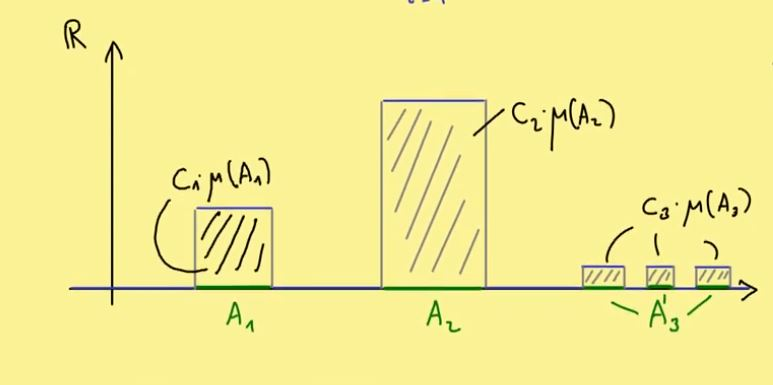
\includegraphics{yt.jpg}

\textbf{Definition}

\[S^{+}:=\{ f: X \rightarrow \mathbb{R}| f: simple \; function, f\geq0\}\]

Properties:

\begin{enumerate}
\def\labelenumi{(\arabic{enumi})}
\item
  \(I(\alpha f + \beta g)=\alpha I(f) +\beta I(g)\), \(\alpha, \beta\geq 0\)
\item
  \(f \leq g \rightarrow I(f) \leq I(g) (monotonicity)\)
\end{enumerate}

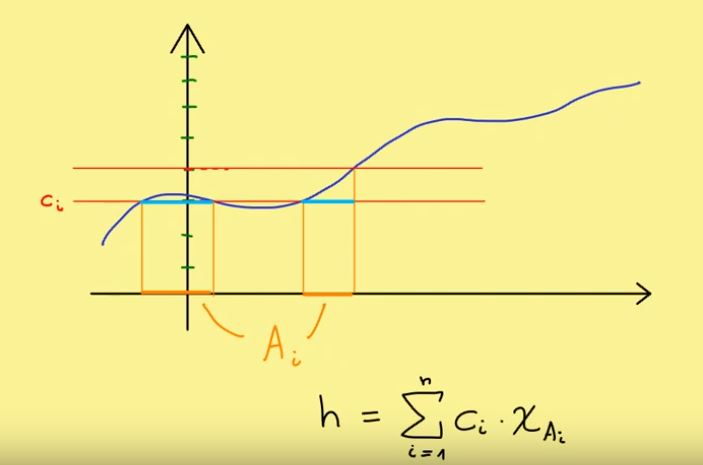
\includegraphics{yt2.jpg}

\textbf{Definitions}

\(f: X \rightarrow [0, \infty) measurable\)

\(\int f d(\mu):=sup \{ I(h) | h \in S^+, h \leq f \}\), in which, \(h = \sum_{i=1}^n c_i x_{A_i}\). We call this Lebesgue integral of \(f\) w.r.t \(\mu\). \(f\) is called \(\mu\)-integral if \(\int_x f d\mu < =\infty\)

\hypertarget{cholesky-decomposition}{%
\chapter{Cholesky decomposition}\label{cholesky-decomposition}}

\hypertarget{example-1}{%
\section{Example 1}\label{example-1}}

Use Cholesky decomposition to generate 1,000 trivariate normal deviates \(X_1, ..., x_{1000}\) with mean \(\mu\) = (−2, 4, 3) and covariance matrix

\[X=\begin{bmatrix}
2 & -1 & 0.5 \\
-1 & 4 & 1 \\
0.5 & 1 & 5 
\end{bmatrix}\]

\begin{Shaded}
\begin{Highlighting}[]
\NormalTok{Nsim =}\StringTok{ }\DecValTok{10}           
\NormalTok{means =}\StringTok{ }\KeywordTok{c}\NormalTok{(}\OperatorTok{-}\DecValTok{2}\NormalTok{,}\DecValTok{4}\NormalTok{,}\DecValTok{3}\NormalTok{)              }
\NormalTok{N_columns =}\StringTok{ }\DecValTok{3}               

\CommentTok{# Generating random standard normal distribution numbers }
\NormalTok{Generated_numbers =}\StringTok{ }\KeywordTok{matrix}\NormalTok{(}\KeywordTok{rnorm}\NormalTok{(N_columns }\OperatorTok{*}\StringTok{ }\NormalTok{Nsim), }\DataTypeTok{nrow =}\NormalTok{ N_columns) }

\CommentTok{# The provided covariance matrix}
\NormalTok{cov_matrix =}\StringTok{ }\KeywordTok{rbind}\NormalTok{(}\KeywordTok{c}\NormalTok{(}\DecValTok{2}\NormalTok{, }\DecValTok{-1}\NormalTok{, }\FloatTok{0.5}\NormalTok{), }\KeywordTok{c}\NormalTok{(}\OperatorTok{-}\DecValTok{1}\NormalTok{, }\DecValTok{4}\NormalTok{, }\DecValTok{1}\NormalTok{), }\KeywordTok{c}\NormalTok{(}\FloatTok{0.5}\NormalTok{, }\DecValTok{1}\NormalTok{, }\DecValTok{5}\NormalTok{))}

\CommentTok{# Cholesky decomposition }
\NormalTok{Cholesky_decom_results =}\StringTok{ }\KeywordTok{chol}\NormalTok{(cov_matrix)    }

\CommentTok{# Data is transformed using the Cholesky decomposition }
\NormalTok{adjusted_data =}\StringTok{ }\KeywordTok{t}\NormalTok{(Generated_numbers) }\OperatorTok\StringTok{ }\NormalTok{Cholesky_decom_results       }

\NormalTok{Final_data =}\StringTok{ }\KeywordTok{t}\NormalTok{(}\KeywordTok{t}\NormalTok{(adjusted_data) }\OperatorTok{+}\StringTok{ }\NormalTok{means)}



\CommentTok{# calculating column means}
\KeywordTok{colMeans}\NormalTok{(Final_data)}
\end{Highlighting}
\end{Shaded}

\begin{verbatim}
## [1] -1.931395  4.499692  2.216270
\end{verbatim}

\begin{Shaded}
\begin{Highlighting}[]
\CommentTok{# calculating column variances}
\KeywordTok{apply}\NormalTok{(Final_data,}\DecValTok{2}\NormalTok{,var)}
\end{Highlighting}
\end{Shaded}

\begin{verbatim}
## [1] 3.189716 1.953063 8.174249
\end{verbatim}

\begin{Shaded}
\begin{Highlighting}[]
\CommentTok{# calculating covariance matrix}
\KeywordTok{cov}\NormalTok{(Final_data)}
\end{Highlighting}
\end{Shaded}

\begin{verbatim}
##           [,1]      [,2]      [,3]
## [1,]  3.189716 -1.433350  3.000417
## [2,] -1.433350  1.953063 -1.655349
## [3,]  3.000417 -1.655349  8.174249
\end{verbatim}

\hypertarget{example-2}{%
\section{Example 2}\label{example-2}}

AR(1) Covariance Matrix with Correlatiion Rho and Variance SigmaSq. Note that, there are only one individual or participant in this data simulation.

\begin{Shaded}
\begin{Highlighting}[]
\NormalTok{n =}\StringTok{ }\DecValTok{10}\NormalTok{;}
\NormalTok{SigmaSq =}\StringTok{ }\DecValTok{5}\NormalTok{;}
\NormalTok{Rho =}\StringTok{ }\FloatTok{0.8}\NormalTok{;}

\NormalTok{V =}\StringTok{ }\KeywordTok{matrix}\NormalTok{(}\KeywordTok{rep}\NormalTok{(n}\OperatorTok{*}\NormalTok{n,}\DecValTok{0}\NormalTok{),n,n);}

\ControlFlowTok{for}\NormalTok{ (i }\ControlFlowTok{in} \DecValTok{1}\OperatorTok{:}\NormalTok{n)}
\NormalTok{\{}
  \ControlFlowTok{for}\NormalTok{ (j }\ControlFlowTok{in}\NormalTok{ i}\OperatorTok{:}\NormalTok{n)}
\NormalTok{  \{}
\NormalTok{    V[i,j]=SigmaSq}\OperatorTok{*}\NormalTok{Rho}\OperatorTok{^}\NormalTok{(j}\OperatorTok{-}\NormalTok{i)}
\NormalTok{    V[j,i]=V[i,j]}
\NormalTok{  \}}
\NormalTok{\}}

\KeywordTok{set.seed}\NormalTok{(}\DecValTok{123}\NormalTok{)}
\NormalTok{random_normal<-}\KeywordTok{rnorm}\NormalTok{(n,}\DecValTok{2}\NormalTok{,}\DecValTok{1}\NormalTok{)}
\CommentTok{#chol(V) %*% random_normal}
\CommentTok{#colSums (chol(V))}
\NormalTok{b2<-}\KeywordTok{t}\NormalTok{(}\KeywordTok{as.matrix}\NormalTok{(random_normal))}\OperatorTok\KeywordTok{chol}\NormalTok{(V)}

\NormalTok{pi =}\StringTok{ }\KeywordTok{exp}\NormalTok{(b2)}\OperatorTok{/}\NormalTok{(}\DecValTok{1} \OperatorTok{+}\StringTok{ }\KeywordTok{exp}\NormalTok{(b2));}

\NormalTok{y<-}\KeywordTok{ifelse}\NormalTok{(pi}\OperatorTok{>}\KeywordTok{runif}\NormalTok{(}\DecValTok{1}\NormalTok{),}\DecValTok{1}\NormalTok{,}\DecValTok{0}\NormalTok{)}

\NormalTok{y}
\end{Highlighting}
\end{Shaded}

\begin{verbatim}
##      [,1] [,2] [,3] [,4] [,5] [,6] [,7] [,8] [,9] [,10]
## [1,]    1    1    1    1    1    1    1    1    1     1
\end{verbatim}

\begin{Shaded}
\begin{Highlighting}[]
\CommentTok{# The code above basically completes the generating job! }
\CommentTok{# The code below is to check }

\NormalTok{b =}\StringTok{ }\NormalTok{b2[}\DecValTok{2}\OperatorTok{:}\NormalTok{n]}
\NormalTok{c =}\StringTok{ }\NormalTok{b2[}\DecValTok{1}\OperatorTok{:}\NormalTok{(n}\DecValTok{-1}\NormalTok{)]}
\KeywordTok{cor}\NormalTok{(b,c)   }
\end{Highlighting}
\end{Shaded}

\begin{verbatim}
## [1] 0.8967058
\end{verbatim}

\begin{Shaded}
\begin{Highlighting}[]
\KeywordTok{sd}\NormalTok{(}\KeywordTok{as.vector}\NormalTok{(b2))}
\end{Highlighting}
\end{Shaded}

\begin{verbatim}
## [1] 3.535119
\end{verbatim}

\begin{Shaded}
\begin{Highlighting}[]
\CommentTok{# note that, you can not use var, as the mean is not zero, but rather it is 2}
\KeywordTok{var}\NormalTok{(}\KeywordTok{as.vector}\NormalTok{(b2))}
\end{Highlighting}
\end{Shaded}

\begin{verbatim}
## [1] 12.49707
\end{verbatim}

\begin{Shaded}
\begin{Highlighting}[]
\CommentTok{#Not sure why the means are not the same ?}
\KeywordTok{mean}\NormalTok{(}\KeywordTok{as.vector}\NormalTok{(b2))}
\end{Highlighting}
\end{Shaded}

\begin{verbatim}
## [1] 10.01925
\end{verbatim}

\begin{Shaded}
\begin{Highlighting}[]
\KeywordTok{mean}\NormalTok{(random_normal)}
\end{Highlighting}
\end{Shaded}

\begin{verbatim}
## [1] 2.074626
\end{verbatim}

\hypertarget{example-3}{%
\section{Example 3}\label{example-3}}

The following code very similar to the code shown above. However, it had only one observation. To illustrate the situation where there are more than one individual (or, participant), I did the code below.

\begin{Shaded}
\begin{Highlighting}[]
\NormalTok{n =}\DecValTok{25}\NormalTok{;   }\CommentTok{#the number of time points}
\NormalTok{m=}\StringTok{ }\DecValTok{15}\NormalTok{;   }\CommentTok{# the number of participants or individuals, whichever ways you would like to think }
\NormalTok{SigmaSq =}\StringTok{ }\DecValTok{5}\NormalTok{;}
\NormalTok{Rho =}\StringTok{ }\FloatTok{0.8}\NormalTok{;}

\NormalTok{filling_numbers<-}\KeywordTok{rep}\NormalTok{(n}\OperatorTok{*}\NormalTok{n,}\DecValTok{0}\NormalTok{)}
\NormalTok{V =}\StringTok{ }\KeywordTok{matrix}\NormalTok{(filling_numbers,n,n);}

\ControlFlowTok{for}\NormalTok{ (i }\ControlFlowTok{in} \DecValTok{1}\OperatorTok{:}\NormalTok{n)}
\NormalTok{\{}
  \ControlFlowTok{for}\NormalTok{ (j }\ControlFlowTok{in}\NormalTok{ i}\OperatorTok{:}\NormalTok{n)}
\NormalTok{  \{}
\NormalTok{    V[i,j]=SigmaSq}\OperatorTok{*}\NormalTok{Rho}\OperatorTok{^}\NormalTok{(j}\OperatorTok{-}\NormalTok{i)}
\NormalTok{    V[j,i]=V[i,j]}
\NormalTok{  \}}
\NormalTok{\}}

\KeywordTok{set.seed}\NormalTok{(}\DecValTok{2345}\NormalTok{)}
\NormalTok{random_normal<-}\KeywordTok{matrix}\NormalTok{(}\KeywordTok{rnorm}\NormalTok{(m}\OperatorTok{*}\NormalTok{n),}\DataTypeTok{nrow =}\NormalTok{ m)}
\CommentTok{#chol(V) %*% random_normal}
\CommentTok{#colSums (chol(V))}
\NormalTok{b2<-random_normal}\OperatorTok\KeywordTok{chol}\NormalTok{(V)}

\NormalTok{pi =}\StringTok{ }\KeywordTok{exp}\NormalTok{(b2)}\OperatorTok{/}\NormalTok{(}\DecValTok{1} \OperatorTok{+}\StringTok{ }\KeywordTok{exp}\NormalTok{(b2));}

\NormalTok{random_unfirom<-}\KeywordTok{matrix}\NormalTok{(}\KeywordTok{runif}\NormalTok{(m}\OperatorTok{*}\NormalTok{n),}\DataTypeTok{nrow =}\NormalTok{ m)}

\NormalTok{y<-}\KeywordTok{ifelse}\NormalTok{(pi}\OperatorTok{>}\NormalTok{random_unfirom,}\DecValTok{1}\NormalTok{,}\DecValTok{0}\NormalTok{)}
\NormalTok{y}
\end{Highlighting}
\end{Shaded}

\begin{verbatim}
##       [,1] [,2] [,3] [,4] [,5] [,6] [,7] [,8] [,9] [,10] [,11] [,12] [,13]
##  [1,]    0    0    0    0    0    0    1    1    1     1     1     0     1
##  [2,]    0    1    1    1    1    1    0    1    0     0     0     0     0
##  [3,]    1    0    0    0    0    1    0    1    0     1     1     0     0
##  [4,]    1    0    0    0    0    0    0    0    1     0     0     0     0
##  [5,]    0    0    0    0    1    0    0    0    0     0     0     0     1
##  [6,]    0    0    1    1    0    0    0    1    0     0     0     0     0
##  [7,]    0    0    0    0    0    1    0    0    1     0     0     0     1
##  [8,]    1    1    1    1    0    0    0    0    0     1     1     0     0
##  [9,]    1    1    1    1    0    1    1    1    0     1     0     0     0
## [10,]    1    0    1    1    1    1    1    1    1     1     0     0     0
## [11,]    1    1    1    1    1    1    1    1    1     0     1     0     0
## [12,]    1    1    1    1    1    1    0    1    1     1     1     1     0
## [13,]    0    1    0    0    0    0    0    0    1     1     1     1     0
## [14,]    1    1    0    1    1    1    1    1    1     0     0     0     0
## [15,]    1    1    0    1    1    1    1    0    0     1     0     0     1
##       [,14] [,15] [,16] [,17] [,18] [,19] [,20] [,21] [,22] [,23] [,24] [,25]
##  [1,]     1     1     1     1     0     1     0     0     1     0     0     0
##  [2,]     0     1     1     1     1     1     0     0     0     1     0     1
##  [3,]     0     1     0     0     1     1     1     1     0     0     1     1
##  [4,]     1     0     0     0     0     0     1     0     1     0     0     0
##  [5,]     0     0     1     1     1     0     1     1     1     0     1     1
##  [6,]     1     1     0     0     1     0     0     1     0     1     1     1
##  [7,]     0     0     0     0     0     1     0     0     1     0     0     0
##  [8,]     0     0     0     0     0     0     0     0     0     1     1     1
##  [9,]     0     1     1     1     0     0     1     0     0     0     0     0
## [10,]     1     1     1     1     1     1     1     1     1     1     1     1
## [11,]     0     0     0     1     0     0     0     0     1     1     1     0
## [12,]     0     0     0     0     1     1     1     0     0     0     1     0
## [13,]     0     1     0     0     0     1     0     1     1     1     1     1
## [14,]     0     0     0     0     1     0     1     0     0     0     0     0
## [15,]     0     0     0     0     0     0     1     0     1     0     0     1
\end{verbatim}

\begin{Shaded}
\begin{Highlighting}[]
\CommentTok{# The code above basically completes the generating job! The code below is to check }

\CommentTok{# The following calcuates variance}
\CommentTok{# calculate variance of each column}
\KeywordTok{mean}\NormalTok{(}\KeywordTok{apply}\NormalTok{(b2, }\DecValTok{2}\NormalTok{, var))}
\end{Highlighting}
\end{Shaded}

\begin{verbatim}
## [1] 4.330903
\end{verbatim}

\begin{Shaded}
\begin{Highlighting}[]
\CommentTok{# calculate variance of each row}
\KeywordTok{mean}\NormalTok{(}\KeywordTok{apply}\NormalTok{(b2, }\DecValTok{1}\NormalTok{, var))}
\end{Highlighting}
\end{Shaded}

\begin{verbatim}
## [1] 3.568107
\end{verbatim}

\begin{Shaded}
\begin{Highlighting}[]
\CommentTok{# The whole table}
\KeywordTok{var}\NormalTok{(}\KeywordTok{as.vector}\NormalTok{(b2))}
\end{Highlighting}
\end{Shaded}

\begin{verbatim}
## [1] 4.299165
\end{verbatim}

\begin{Shaded}
\begin{Highlighting}[]
\CommentTok{# The following code calculates the correlation }
\NormalTok{b =}\StringTok{ }\NormalTok{b2[,}\DecValTok{2}\OperatorTok{:}\NormalTok{n]}
\NormalTok{c =}\StringTok{ }\NormalTok{b2[,}\DecValTok{1}\OperatorTok{:}\NormalTok{(n}\DecValTok{-1}\NormalTok{)]}

\NormalTok{collected_cor<-}\KeywordTok{rep}\NormalTok{(}\DecValTok{0}\NormalTok{,m}\DecValTok{-1}\NormalTok{) }\CommentTok{#creating an empty vector to collect correlation. }
\ControlFlowTok{for}\NormalTok{ (i }\ControlFlowTok{in} \DecValTok{1}\OperatorTok{:}\NormalTok{(m}\DecValTok{-1}\NormalTok{))}
\NormalTok{\{collected_cor[i]<-}\KeywordTok{cor}\NormalTok{(b[i,],c[i,])\}}
\NormalTok{collected_cor}
\end{Highlighting}
\end{Shaded}

\begin{verbatim}
##  [1] 0.8473037 0.7065013 0.6376223 0.5481540 0.7851062 0.6576329 0.4844481
##  [8] 0.6950847 0.6731673 0.6409116 0.7966547 0.7184030 0.8001861 0.7913736
\end{verbatim}

\begin{Shaded}
\begin{Highlighting}[]
\KeywordTok{mean}\NormalTok{(collected_cor)}
\end{Highlighting}
\end{Shaded}

\begin{verbatim}
## [1] 0.6987535
\end{verbatim}

\begin{Shaded}
\begin{Highlighting}[]
\KeywordTok{mean}\NormalTok{(y)}
\end{Highlighting}
\end{Shaded}

\begin{verbatim}
## [1] 0.456
\end{verbatim}

\begin{Shaded}
\begin{Highlighting}[]
\KeywordTok{log}\NormalTok{(}\KeywordTok{mean}\NormalTok{(y)}\OperatorTok{/}\NormalTok{(}\DecValTok{1}\OperatorTok{-}\KeywordTok{mean}\NormalTok{(y)))}
\end{Highlighting}
\end{Shaded}

\begin{verbatim}
## [1] -0.1764564
\end{verbatim}

\begin{Shaded}
\begin{Highlighting}[]
\CommentTok{# It will always get a value close to zero, since we set the mean to be zero when simulating the data}
\end{Highlighting}
\end{Shaded}

\backmatter
  \bibliography{book.bib,packages.bib}

\end{document}
